\newpage
\section{Transformée de Fourier}
Ce qu'on a vu jusqu'à maintenant fonctionne pour des fonctions périodiques, mais qu'arrive-t-il lorsqu'on tente d'étendre cela à des fonctions qui ne le sont pas? En d'autres mots, pour une fonction qui a une période infinie, comment se comportent nos précédentes trouvailles? Pour cela, il faut regarder dans la limite où $T \rightarrow \infty$. 

\subsection{Dérivation}
On commence par recopier (\ref{eq_serie_fourier_exp}) et (\ref{eq_coeffs_cn}) en changeant les bornes d'intégration pour (\ref{eq_coeffs_cn}), ce qu'on peut faire par (\ref{eq_int_sym}).

\begin{equation}
    f(x) = \sum_{n = -\infty}^{\infty}c_ne^{2\pi inx/T} \ \text{ où } \ c_n = \frac{1}{T}\int_{-T/2}^{T/2}f(x)e^{-2\pi inx/T}dx
    \label{eq_serie_fourier_exp_v2}
\end{equation}

Soit $\omega_n = \frac{2\pi n}{T}$ la fréquence angulaire de l'exponentielle complexe pour un $n$ donné. Alors, la différence entre deux $\omega_n$ successifs est $\Delta \omega_n = \frac{2\pi}{T}\Delta n = \frac{2\pi}{T}$. Dans la limite où $T \rightarrow \infty$, $\Delta \omega_n$ est infinitésimale et $\omega_n$ devient une variable continue $\omega$. Sachant cela, on effectue quelques manipulations sur (\ref{eq_serie_fourier_exp_v2}). D'abord, on peut dire que

\begin{equation*}
    f(x) = \sum_{n = -\infty}^{\infty}c_ne^{2\pi inx/T} \cdot 1 = \sum_{n = -\infty}^{\infty}c_ne^{i\omega_nx} \Delta n = \sum_{n = -\infty}^{\infty}\left(c_n\frac{T}{2\pi}\right)e^{i\omega_nx}\Delta \omega_n  
\end{equation*}

Puis, dans la limite où la période est infinie, on a 

\begin{equation*}
    f(x) = \lim_{T\rightarrow\infty}\sum_{n = -\infty}^{\infty}\left(c_n\frac{T}{2\pi}\right)e^{i\omega_nx}\Delta \omega_n = \lim_{T\rightarrow\infty}\sum_{n = -\infty}^{\infty}\left(\frac{1}{2\pi}\int_{-T/2}^{T/2}f(x)e^{-i\omega_nx}dx\right) e^{i\omega_nx}\Delta \omega_n
\end{equation*}
\begin{equation}
    = \frac{1}{2\pi}\int_{-\infty}^{\infty}\left(\int_{-\infty}^{\infty}f(x)e^{-i\omega x}dx\right)e^{i\omega x}d\omega = \frac{1}{2\pi}\int_{-\infty}^{\infty}c(\omega)e^{i\omega x}d\omega 
    \label{eq_TFI}
\end{equation}

où on pose 

\begin{equation}
    c(\omega) = \int_{-\infty}^{\infty}f(x)e^{-i\omega x}dx
    \label{eq_TF}
\end{equation}

Comme auparavant, on trouve un coefficient $c(\omega)$ qui nous dit "combien" il y a de la fréquence angulaire $\omega$ dans $f(x)$. En fait, (\ref{eq_TF}) va être ce qu'on appelle la transformée de Fourier (TF) de $f(x)$. D'un autre côté, (\ref{eq_TFI}) correspond à la transformée de Fourier inverse (TFI), parce qu'elle permet depuis les fréquences angulaires de reconstruire $f(x)$. 




Comme pour une série de Fourier, il existe des conditions pour qu'une TF soit juste. Naturellement, comme une TF est une extension d'une série de Fourier, on ne fait qu'étendre les conditions suffisantes vues précédemment.

\begin{enumerate}
    \item $\int_{-\infty}^{\infty}\abs{f(x)}dx < \infty$.
    \item Sur tout intervalle fini de $f(x)$, il y a un nombre fini d'extremums. 
    \item Sur tout intervalle fini de $f(x)$, il y a un nombre fini de discontinuités et elles ont une amplitude finie.
\end{enumerate}

Par ailleurs, bien que la TF soit à la base pour les fonctions qui ne sont pas périodiques, elle s'applique tout de même aux fonctions périodiques puisqu'elles se répètent techniquement aussi à l'infini. Finalement, le facteur $\frac{1}{2\pi}$ aurait pu être déplacé à l'intéreur de $c(\omega)$ si on le voulait. En fait, ce choix dépend des auteurs mais rien ne change mathématiquement.

\subsection{Pulse rectangulaire}
Soit un pulse rectangulaire décrit par $\text{Rect}(x) = \begin{cases}
    A & \text{si } \abs{x} < d/2 \\
    0 & \text{sinon}
\end{cases}$. 

\begin{figure}[H]
    \centering
        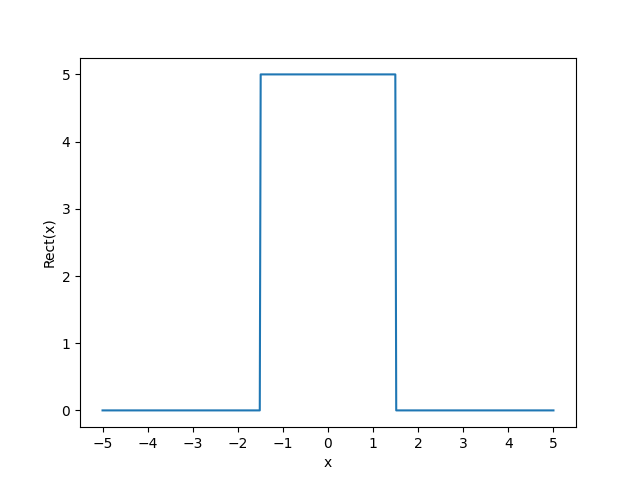
\includegraphics[width=0.5\textwidth]{images/ch3/pulse_rectangulaire.png}
    \caption{Pulse rectangulaire $(A = 5, d = 3)$}
    \label{fig_pulse_rect}
    \end{figure}

Par (\ref{eq_TF}), 

\begin{equation*}
    c(\omega) = \int_{-\infty}^{\infty}\text{Rect}(x)e^{-i\omega x}dx = \int_{-d/2}^{d/2}Ae^{-i\omega x}dx = A\int_{-d/2}^{d/2}\left(\cos(\omega x) - i\sin(\omega x)\right)dx
\end{equation*}
\begin{equation*}
    = A\int_{-d/2}^{d/2}\underbrace{\cos(\omega x)}_\text{paire}dx - iA\int_{-d/2}^{d/2}\underbrace{\sin(\omega x)}_\text{impaire}dx = 2A\int_{0}^{d/2}\cos(\omega x)dx = \frac{2A}{\omega}\sin(\frac{d\omega}{2})
\end{equation*}

\begin{figure}[H]
    \centering
        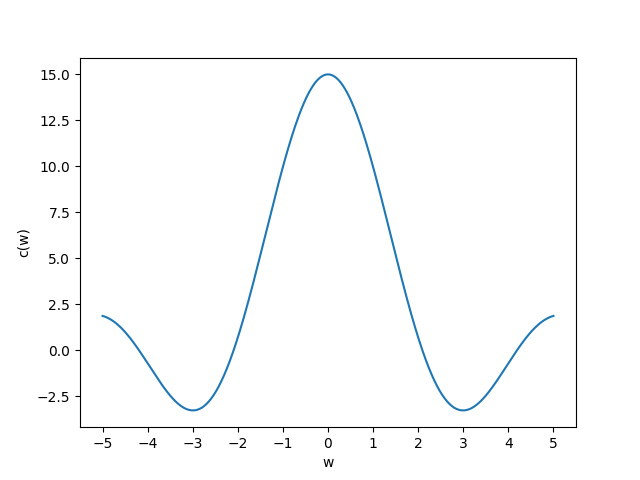
\includegraphics[width=0.48\textwidth]{images/ch3/coeff_pulse_rectangulaire.png}
    \caption{Les premiers $c(\omega)$ pour le pulse rectangulaire ($A = 5, d = 3$)}
    \label{fig_TF_pulse_rect}
    \end{figure}

% \begin{figure}[H]
%     \centering
%         
\includegraphics[width=0.48\textwidth]{images/ch3/magnitude.png}
%         
\includegraphics[width=0.48\textwidth]{images/ch3/phase.png}
%     \caption{Spectre de magnitude (à gauche) et de phase (à droite) des premiers $c(\omega)$ ($A = 5, d = 3$)}
%     \label{fig_magn_phase_pulse_rect}
%     \end{figure}

% Là aussi, on peut montrer que $c(-\omega) = c^*(\omega) \iff r(-\omega)e^{i\theta(-\omega)} = r(\omega)e^{-i\theta(\omega)} \iff r(-\omega) = r(\omega) \ \text{ et } \ \theta(-\omega) = -\theta(\omega)$. Ainsi, le spectre de magnitude est symétrique par rapport à l'origine et le spectre de phase est antisymétrique par rapport à l'origine. À la figure \ref{fig_magn_phase_pulse_rect}, le spectre de phase n'a pas l'air antisymétrique, mais il l'est implicitement sachant que $e^{i\pi} = e^{-i\pi}$.

Par (\ref{eq_TFI}),

\begin{equation*}
    \text{Rect}(x) = \frac{A}{\pi}\int_{-\infty}^{\infty}\frac{\sin(\frac{d\omega}{2})}{\omega}e^{i\omega x}d\omega = \frac{2A}{\pi}\int_{0}^{\infty}\frac{\sin(\frac{d\omega}{2})\cos(\omega x)}{\omega}d\omega
\end{equation*}

en utilisant la formule d'Euler et la parité des fonctions en jeu. Pour vérifier que cela converge bien, il faudrait évaluer l'intégrale, ce qui ne semble pas facile à faire. On peut l'approximer, par exemple, en prenant des bornes d'intégration $\left[0, b\right]$ qui tendent progressivement vers $[0, \infty)$. Les figures ci-dessous présentent cette approximation avec différentes bornes d'intégration. Naturellement, on voit que plus les bornes tendent vers $[0, \infty)$, plus on se rapproche du vrai pulse rectangulaire. 

\begin{figure}[H]
    \centering
        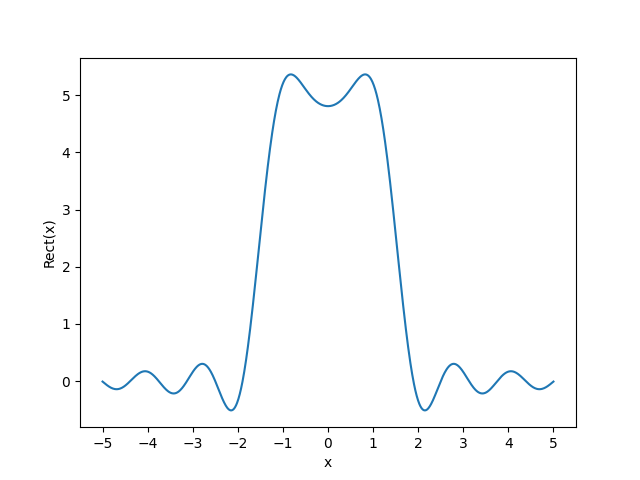
\includegraphics[width=0.48\textwidth]{images/ch3/borne_5.png}
        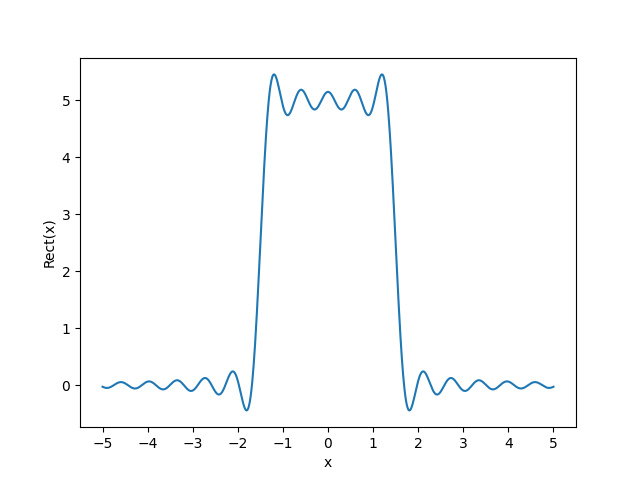
\includegraphics[width=0.48\textwidth]{images/ch3/borne_10.png}
    \caption{TFI de Rect$(x)$ ($A=5, d=3$) avec bornes $[0, 5]$ (à gauche) et $[0, 10]$ (à droite)}
    \label{fig_TFI_pulse_rect_1}
    \end{figure}

    \begin{figure}[H]
        \centering
            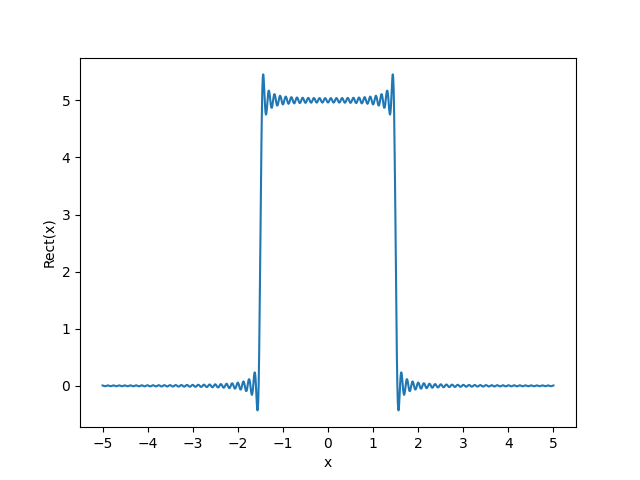
\includegraphics[width=0.48\textwidth]{images/ch3/borne_50.png}
            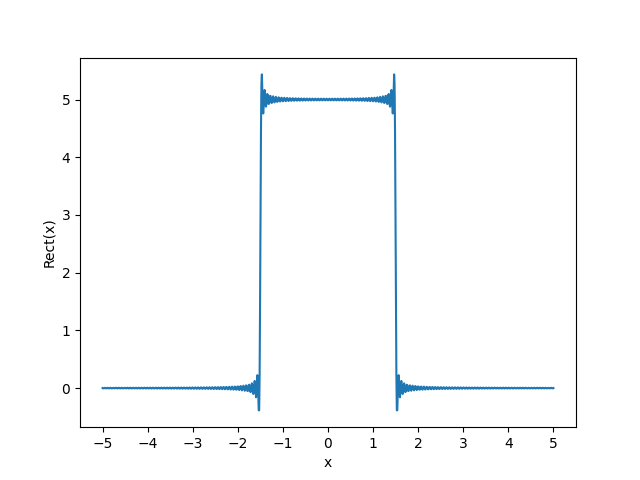
\includegraphics[width=0.48\textwidth]{images/ch3/borne_100.png}
        \caption{TFI de Rect$(x)$ ($A=5, d=3$) avec bornes $[0, 50]$ (à gauche) et $[0, 100]$ (à droite)}
        \label{fig_TFI_pulse_rect_2}
        \end{figure}

\subsection{Propriétés}
La transformée de Fourier possède plusieurs propriétés qui peuvent grandement faciliter les calculs. En voici quelques unes.

\subsubsection{Linéarité}
Soient deux fonctions $f(x)$ et $g(x)$ ayant une TF ainsi que $a,b \in \mathbb{C}$. Alors,

\begin{equation}
    \text{TF}\left(af(x) + bg(x)\right) = a \text{TF}\left(f(x)\right) + b \text{TF}\left(g(x)\right)
    \label{eq_linearite_TF}
\end{equation}

Preuve :

\begin{equation*}
    \text{TF}\left(af(x) + bg(x)\right) = \int_{-\infty}^{\infty}\left(af(x) + bg(x)\right)e^{-i\omega x}dx = a\int_{-\infty}^{\infty}f(x)e^{-i\omega x}dx + b\int_{-\infty}^{\infty}g(x)e^{-i\omega x}dx
\end{equation*}
\begin{equation*}
    = a \text{TF}\left(f(x)\right) + b \text{TF}\left(g(x)\right)
\end{equation*}

\subsubsection{Déplacement en temps/position}
Soient une fonction $f(x)$ ayant une TF ainsi que $x_0 \in \mathbb{R}$. Alors,

\begin{equation}
    \text{TF}\left(f(x-x_0)\right) = e^{-i\omega x_0}\text{TF}\left(f(x)\right)
    \label{eq_deplacement_temps_TF}
\end{equation}

Preuve :

\begin{equation*}
    \text{TF}\left(f(x-x_0)\right) = \int_{-\infty}^{\infty}f(x-x_0)e^{-i\omega x}dx = \int_{-\infty}^{\infty}f(x')e^{-i\omega (x'+x_0)}dx' = e^{-i\omega x_0}\int_{-\infty}^{\infty}f(x')e^{-i\omega x'} dx'
\end{equation*}
\begin{equation*}
    = e^{-i\omega x_0}\text{TF}\left(f(x)\right)
\end{equation*}

\subsubsection{Déplacement du spectre de fréquences}
Soient une fonction $f(x)$ ayant une TF ainsi que $\omega_0 \in \mathbb{R}$. Alors,

\begin{equation}
    \text{TF}\left(e^{i\omega_0 x}f(x)\right) = \text{TF}(f(x)) \text{ décalée de $\omega_0$ à gauche}
\end{equation}

Preuve : 

\begin{equation*}
    \text{TF}\left(e^{i\omega_0 x}f(x)\right) =  \int_{-\infty}^{\infty}e^{i\omega_0 x}f(x)e^{-i\omega x}dx = \int_{-\infty}^{\infty}f(x)e^{-i(\omega-\omega_0)x}dx = \text{TF}(f(x)) \text{ décalée de $\omega_0$ à gauche}
\end{equation*}

